\documentclass[a4paper]{article}

%% Language and font encodings
\usepackage[english]{babel}
\usepackage[utf8x]{inputenc}
\usepackage[T1]{fontenc}

%% Sets page size and margins
\usepackage[a4paper,top=3cm,bottom=2cm,left=3cm,right=3cm,marginparwidth=1.75cm]{geometry}

%% Useful packages
\usepackage{amsmath}
\usepackage{graphicx}
\usepackage[colorinlistoftodos]{todonotes}
\usepackage[colorlinks=true, allcolors=blue]{hyperref}
\usepackage{braket}
\title{QM Problems}
\author{Anoop Chandran -- Lorenzo Fant}

\begin{document}
\maketitle


\section{A. Solid Argon With LJ Potential}

\subsection{Lattice Parameters}
From the general expression of the Lennard-Jones potential
\begin{equation}
V(r) = 4\epsilon\left(\left(\frac{\sigma}{r}\right)^12-\left(\frac{\sigma}{r}\right)^6\right)
\end{equation}
We can easily find the minimum finding the zero of the first derivative.
\begin{equation}
r_0 = 2^{\frac{1}{6}}\sigma
\end{equation}
and, substituting it into the potential expression we find
\begin{equation}
V(r_0) = -\epsilon
\end{equation}
From these two expressions we can deduce $\sigma = \frac{3.758}{2^{\frac{1}{6}}}$\AA and $\epsilon = 99.55 cm^{-1}$
\subsection{Crystal Structures}
Knowing the expression for the Lennard-Jones potential we can derive an approximate value of the energy of different lattice structures by numerically summing the potential energy contributions of the neighbours.
\begin{figure}[h]
    \centering
    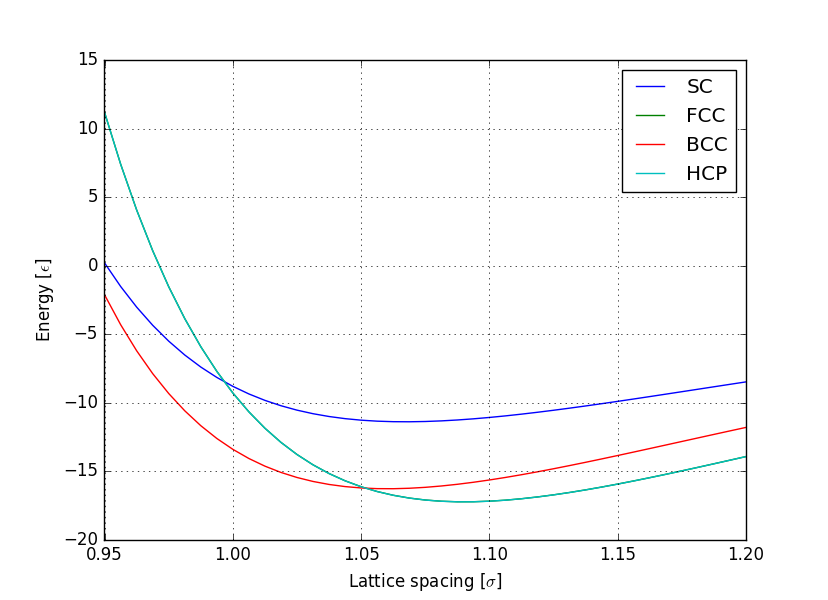
\includegraphics[width=9cm]{energy_lattice_spacing.png}
    \caption{\it \label{en(spacing)}Energy of the atoms in the lattice as a function of the lattice spacing for four possible lattices: Simple Cubic (Blue), Face Centered (Green), Body Centered (Red), hexagonal Cenered (Light blue)}
    \end{figure}
    
Doing so for the $14^3$ closest neighbours we found the following values for the required structures
\begin{eqnarray*}
&spacing&energy\\
sc&1.066\sigma&-11.36\epsilon\\
bcc&1.069\sigma&-16.45\epsilon\\
fcc&1.090\sigma&-17.2160\epsilon\\
hcp&1.090\sigma&-17.2192\epsilon
\end{eqnarray*}
We thus found that the energetically favorable configuration is the $hcp$ one by a factor of $0.01\%$ with respect to the $fcc$.
This is in agreement with re results found in the litterature ref{crystal}. 
In the same reference it is also pointed out that despite $hcp$ configuration being lower in energy, the one that more easily appears in nature is the $fcc$ one.
We here try to justify such a result without considering, as done in ref{crystal}, impurities.\\
We tried instead to consider the behaviour of the energy in the minimum when some random noise is present in the lattice, displacing the positions of the atoms.
We looked at the behaviour of the energy as a function of the amplitude of the noise averaging over $10^4$ different realizations of the system with a Gaussian random displacement of amplitude $d$.

\begin{figure}[ht]
    \centering
    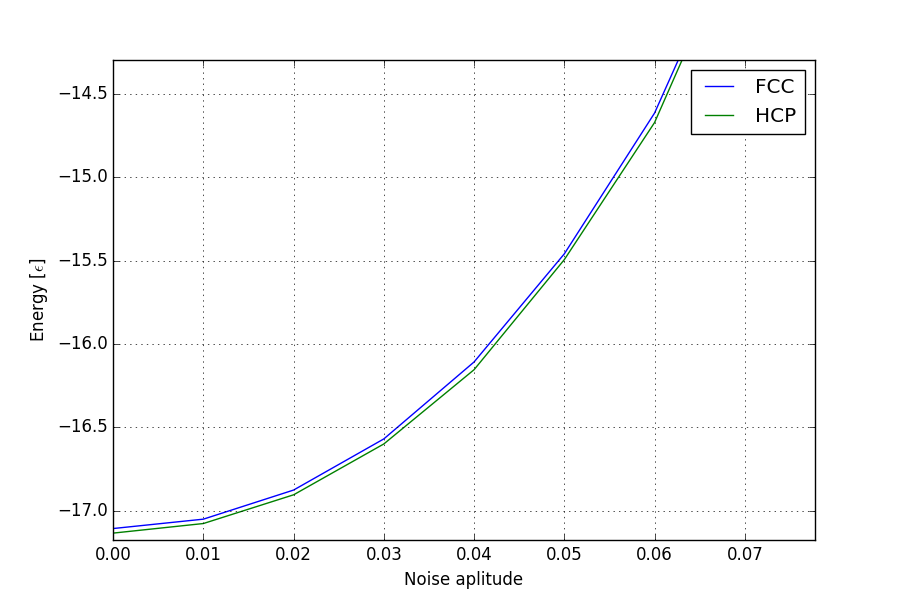
\includegraphics[width=9cm]{energy_noise.png}
    \caption{\it \label{noise}Energy of the minima obtained above for FCC and HCP lattices as a function of the amplitude of a random noise displacing the atoms positions}
    \end{figure}

We can see that there is no crossing between the two energies and thus it the fact that the "fcc" structure is prefererred in nature cannot be explained in this way.

\subsection{Spectrum of the HCP}

In the case of the hcp configuration the cell can be easily identified through the three vectors of coordinates\\
\begin{minipage}{0.3\textwidth}
\centering
\begin{equation*}
R_1 =
\begin{bmatrix}
	1 \\
    0 \\
    0 \\
    
\end{bmatrix}
\end{equation*}

\end{minipage}
\begin{minipage}{0.3\textwidth}
\centering
\begin{equation*}
R_2 =
\begin{bmatrix}
    \frac{1}{2} \\
    \frac{\sqrt{3}}{2}  \\
    0 \\
\end{bmatrix}
\end{equation*}
\end{minipage}
\begin{minipage}{0.3\textwidth}
\centering
\begin{equation*}
R_3 =
\begin{bmatrix}
    \frac{1}{2} \\
    \frac{1}{2\sqrt{3}}  \\
    \sqrt{\frac{2}{3}} \\
\end{bmatrix}
\end{equation*}
\end{minipage}



and that of the corresponding reciprocal lattice vectors can be constructed from those above and their coordinates are \\
\begin{minipage}{0.3\textwidth}
    \centering
    \begin{equation*}
    G_1 =
    \begin{bmatrix}
        0 \\
        0 \\
        \sqrt{\frac{3}{2}}\pi \\
        
    \end{bmatrix}
    \end{equation*}
    
    \end{minipage}
    \begin{minipage}{0.3\textwidth}
    \centering
    \begin{equation*}
    G_2 =
    \begin{bmatrix}
        \frac{1}{2} \\
        \frac{\sqrt{3}}{2}  \\
        0 \\
    \end{bmatrix}
    \end{equation*}
    \end{minipage}
    \begin{minipage}{0.3\textwidth}
    \centering
    \begin{equation*}
    G_3 =
    \begin{bmatrix}
        \frac{1}{2} \\
        \frac{1}{2\sqrt{3}}  \\
        \sqrt{\frac{2}{3}} \\
    \end{bmatrix}
    \end{equation*}
    \end{minipage}
    \subsection{Spectrum of the FCC}

    In the case of the hcp configuration the cell can be easily identified through the three vectors of coordinates\\
    \begin{minipage}{0.3\textwidth}
    \centering
    \begin{equation*}
    R_1 =
    \begin{bmatrix}
        1 \\
        0 \\
        0 \\
        
    \end{bmatrix}
    \end{equation*}
    
    \end{minipage}
    \begin{minipage}{0.3\textwidth}
    \centering
    \begin{equation*}
    R_2 =
    \begin{bmatrix}
        \frac{1}{2} \\
        \frac{\sqrt{3}}{2}  \\
        0 \\
    \end{bmatrix}
    \end{equation*}
    \end{minipage}
    \begin{minipage}{0.3\textwidth}
    \centering
    \begin{equation*}
    R_3 =
    \begin{bmatrix}
        \frac{1}{2} \\
        \frac{1}{2\sqrt{3}}  \\
        \sqrt{\frac{2}{3}} \\
    \end{bmatrix}
    \end{equation*}
    \end{minipage}
    
    
    
    and that of the corresponding reciprocal lattice vectors can be constructed from those above and their coordinates are \\
    \begin{minipage}{0.3\textwidth}
        \centering
        \begin{equation*}
        G_1 =
        \begin{bmatrix}
            0 \\
            0 \\
            \sqrt{\frac{3}{2}}\pi \\
            
        \end{bmatrix}
        \end{equation*}
        
        \end{minipage}
        \begin{minipage}{0.3\textwidth}
        \centering
        \begin{equation*}
        G_2 =
        \begin{bmatrix}
            \frac{1}{2} \\
            \frac{\sqrt{3}}{2}  \\
            0 \\
        \end{bmatrix}
        \end{equation*}
        \end{minipage}
        \begin{minipage}{0.3\textwidth}
        \centering
        \begin{equation*}
        G_3 =
        \begin{bmatrix}
            \frac{1}{2} \\
            \frac{1}{2\sqrt{3}}  \\
            \sqrt{\frac{2}{3}} \\
        \end{bmatrix}
        \end{equation*}
        \end{minipage}
    
From this we can construct the Brillouin zone which corresponds to the Wigner-Seitz cell in K-space\\

The $2P_{x}, 2P_{y}$, and 2S orbitals undergo $SP_{2}$ hybridization and the electrons form strong covalent sigma bonds with the neighbouring sites. So it is sufficient to consider only the $P_{z}$ orbitals in the tight binding calculation

From Bloch's theorem it follows that our wave function will be of the form

\begin{eqnarray}
    \ket{\psi}&=&\sum_{R}\exp(iKR)(\exp(ika_{1})c_{1}\ket{R,1} + \exp(ika_{1})c_{2}\ket{R,2} )\\
	\ket{\psi}&=&\sum_{R}\exp(i\vec{K}\vec{R})(b_{1}\ket{R,1} + b_{2}\ket{R,2} )
\end{eqnarray}


Where $\vec{R} = n\vec{R1} + m\vec{R2} $  with $m,n \in Z$


We solve the Eigenvalue problem and project onto the kets corresponding to the cell R =(0,0) 
\begin{eqnarray}
\bra{0,1}H\ket{\psi}&=&E\bra{0,1}\ket{\psi}\\
\bra{0,2}H\ket{\psi}&=&E\bra{0,2}\ket{\psi}
\end{eqnarray}

Expanding the above equation gives us two linear equations in two variables. 
\begin{eqnarray}
(E-e_{c})b_1  +  t(1 + \exp(-ikR_{1}) + \exp(-ikR_{2}))b_2 & = & 0\\
 t(1 + \exp(ikR_{1})b_1  +     \exp(ikR_{2})) + (E-e_{c})b_2 & = &  0
\end{eqnarray}

from this we find that the band structure is

\begin{equation}
E = e_c \pm t\sqrt{(1 + \cos(\vec{k}\vec{R_{1}}) + \cos(\vec{k}\vec{R_{2}}) )^2  + ( \sin(\vec{k}\vec{R_{1}}) + \sin(\vec{k}\vec{R_{2}}) )^2  }
\end{equation}

From the Eigenvalues we can eventually find the dependence of the $b_1,b_2$ factors in the wave function on the parameters of the system as 
\begin{equation}
b_1 = \sqrt{\frac{1}{1+a}}
\hspace{1cm}
b_2 = \sqrt{\frac{a}{1+a}}
\end{equation}
where
\begin{equation*}
a = \frac{1 + e^{i\vec{k}\vec{R_{1}}} + e^{i\vec{k}\vec{R_{2}}}}{1 + e^{-i\vec{k}\vec{R_{1}}} + e^{-i\vec{k}\vec{R_{2}}}}
\end{equation*}

Assuming the value of t = -2.5 and measuring our energy from $e_{c}$
we obtain the plot shown below
\begin{figure}[h]

\centering
\caption{\label{fig:frog}3d plot of the band structure of Graphene}
\end{figure}
\clearpage
We observe the existence of Dirac cones,at the points where the two bands touch with linear dispersion. To see this more clearly we plot The Energy along the line $K_{y} = \frac{K_{x}}{\sqrt{3}}$

\begin{figure}[h]
\centering
\caption{\label{fig:frog}2d plot of Graphene spectrum along the $K_{y}=\frac{K{x}}{\sqrt{3}}$ }
\end{figure}

We then numerically calculated the density of states as a function of the energy obtaining the function plotted below
\begin{figure}[h!]
\centering
\caption{\label{fig:frog}Density of states against Energy}
\end{figure}

We can see the linear dependence of $n(E)$ for $E \sim 0$. To see instead the behavior on the function around the divergence we decided to plot it as a function of $y_1:=\log(E-E_{0})$ for $E>E_0$ and $y_2:=\log(E_0-E)$ for $E<E_0$. Where $E_{0} = 2.479 $ is the Energy that maximizes the density of states.

\begin{figure}[h!]
\centering
\caption{\label{fig:frog}DOS against $\log(E-E_{0})$}
\end{figure}

We can here observe near linear behavior for $y_i\rightarrow-\infty$.
This clearly shoes the logarithmic dependence of the divergence.

\section{Boron-Nitride Model}

\begin{figure}[h!]
\centering
\caption{\label{BN} BN hexagonal mono layer sheet}
\end{figure}
The unit cell, lattice vectors and reciprocal lattice vectors are equivalent to that of graphene and are written below Fig.(\ref{BN}). Their coordinates are \\
\begin{minipage}{0.5\textwidth}
\centering
\begin{equation*}
R_1 =
\begin{bmatrix}
	\frac{3}{2} \\
    \frac{\sqrt{3}}{2}  \\
    
\end{bmatrix}
\end{equation*}

\end{minipage}
\begin{minipage}{0.5\textwidth}
\centering
\begin{equation*}
R_2 =
\begin{bmatrix}
    \frac{3}{2} \\
    \frac{-\sqrt{3}}{2}  \\
\end{bmatrix}
\end{equation*}
\end{minipage}



and that of the corresponding reciprocal lattice vectors can be constructed from those above and their coordinates are \\
\begin{minipage}{0.5\textwidth}
\centering
\begin{equation*}
G_1 =
\begin{bmatrix}
    \frac{2\pi}{3} \\
    \frac{2\pi}{\sqrt{3}} \\
\end{bmatrix}
\end{equation*}


\end{minipage}
\begin{minipage}{0.5\textwidth}
\centering
\begin{equation*}
G_2 =
\begin{bmatrix}
    \frac{2\pi}{3} \\
    -\frac{2\pi}{\sqrt{3}} \\
\end{bmatrix}
\end{equation*}
\end{minipage}

From this we can construct the Brillouin zone which corresponds to the Wigner-Seitz cell in K-space\\

From Bloch's theorem it follows that our wave function will be of the form

\begin{eqnarray}
    \ket{\psi}&=&\sum_{R}\exp(iKR)(\exp(ika_{1})c_{1}\ket{R,1} + \exp(ika_{1})c_{2}\ket{R,2} )\\
	\ket{\psi}&=&\sum_{R}\exp(i\vec{K}\vec{R})(b_{1}\ket{R,1} + b_{2}\ket{R,2} )
\end{eqnarray}


Where $\vec{R} = n\vec{R1} + m\vec{R2} $  with $m,n \in Z$

We solve the Eigenvalue problem and project onto the kets corresponding to the cell R =(0,0) 
\begin{eqnarray}
\bra{0,1}H\ket{\psi}&=&E\bra{0,1}\ket{\psi}\\
\bra{0,2}H\ket{\psi}&=&E\bra{0,2}\ket{\psi}
\end{eqnarray}

Writing explicitly the above equations gives us two linear equations in two variables. 
\begin{eqnarray}
(E-e_{c} + \frac{\Delta}{2})b_1  +  t(1 + \exp(-ikR_{1}) + \exp(-ikR_{2}))b_2 & = & 0\\
 t(1 + \exp(ikR_{1})b_1 + \exp(ikR_{2})) + (E-e_{c}-\frac{\Delta}{2})b_2 & = &  0
\end{eqnarray}

from this we find that the band structure is

\begin{equation}
E = e_{c}  \pm  \sqrt{\frac{\Delta^2}{4} +t^2 ((1 + \cos(\vec{k}\vec{R_{1}}) + \cos(\vec{k}\vec{R_{2}}) )^2  + t^2 (( \sin(\vec{k}\vec{R_{1}}) + \sin(\vec{k}\vec{R_{2}}) )^2  }
\end{equation}
assuming the value of t = -2.5 and measuring our energy from $e_{c}$ and $\Delta = 6.1$(i.e the difference in first ionization energies between Boron and nitrogen)
we obtain the plot shown below
\begin{figure}[h]

\centering
\caption{\label{fig:frog}3d plot of the band structure of Boron Nitride}
\end{figure}

We do not observe the existence of Dirac cones. plotting The Energy along the line $K_{y} = \frac{K_{x}}{\sqrt{3}}$ we observe a band gap of roughly 5ev
\begin{figure}[h]
\centering
\caption{\label{bn band}2d plot of Boron Nitride lowest band along the $K_{y}=\frac{K{x}}{\sqrt{3}}$ }
\end{figure}\\


\begin{figure}[h]
\centering
\caption{\label{bn density}Density of states }
\end{figure}

\newpage
\section{Boron, Carbon, Nitrogen Model}

\begin{figure}[h!]
\centering
\caption{\label{cbn} \it The structure of the system under examination. Atoms are shown as: Black-Carbon, Blue-Boron, Red-Nitrogen. Light gray lines are drown just to emphasize the honeycomb structure of the cells.}
\end{figure}
The cell, since the lattice is, as before, honeycomb-shaped is identified by the two vectors used up to know, just scaled by a common factor that doesn't affect the physics, as shown in Fig.(\ref{cbn}). Their coordinates are \\
\begin{minipage}{0.5\textwidth}
\centering
\begin{equation*}
R_1 =
\begin{bmatrix}
	3 \\
    \sqrt{3}  \\
    
\end{bmatrix}
\end{equation*}

\end{minipage}
\begin{minipage}{0.5\textwidth}
\centering
\begin{equation*}
R_2 =
\begin{bmatrix}
    3 \\
   -\sqrt{3}  \\
\end{bmatrix}
\end{equation*}
\end{minipage}



and that of the corresponding reciprocal lattice vectors can be constructed from those above and their coordinates are \\
\begin{minipage}{0.5\textwidth}
\centering
\begin{equation*}
G_1 =
\begin{bmatrix}
    \frac{\pi}{3} \\
    \frac{\pi}{\sqrt{3}} \\
\end{bmatrix}
\end{equation*}


\end{minipage}
\begin{minipage}{0.5\textwidth}
\centering
\begin{equation*}
G_2 =
\begin{bmatrix}
    \frac{\pi}{3} \\
    -\frac{\pi}{\sqrt{3}} \\
\end{bmatrix}
\end{equation*}
\end{minipage}

From this we can construct the Brillouin zone which corresponds to the Wigner-Seitz cell in K-space\\

From Bloch's theorem it follows that our wave function will be of the form

\begin{equation}
\ket{\psi}=\sum_{R}\exp(i\vec{K}\vec{R})(b_{1}\ket{R,1} + b_{2}\ket{R,2}+
b_{3}\ket{R,3} + b_{4}\ket{R,4}+b_{5}\ket{R,5} +b_{6}\ket{R,6} +b_{7}\ket{R,7}+b_{8}\ket{R,8} )
\end{equation}


Where $\vec{R} = n\vec{R1} + m\vec{R2} $  with $m,n \in Z$

We solve the Eigenvalue problem and project onto the kets corresponding to the cell R =(0,0) 
%\begin{eqnarray}
%\bra{0,1}H\ket{\psi}&=&E\bra{0,1}\ket{\psi}\\
%\bra{0,2}H\ket{\psi}&=&E\bra{0,2}\ket{\psi}\\
%\bra{0,3}H\ket{\psi}&=&E\bra{0,3}\ket{\psi}\\
%\bra{0,4}H\ket{\psi}&=&E\bra{0,4}\ket{\psi}\\
%\bra{0,5}H\ket{\psi}&=&E\bra{0,5}\ket{\psi}\\
%\bra{0,6}H\ket{\psi}&=&E\bra{0,6}\ket{\psi}\\
%\bra{0,7}H\ket{\psi}&=&E\bra{0,7}\ket{\psi}\\
%\bra{0,8}H\ket{\psi}&=&E\bra{0,8}\ket{\psi}
%\end{eqnarray}



This brings us to an Hamiltonian representation of the following form

\[ \left( \begin{array}{cccccccc}
e_c & 0 & -t_{CN} & 0 & -t_{CN}e^{-i\vec{k}\vec{R_1}} & 0 & -t_{CN}e^{-i\vec{k}\vec{R_2}} & 0\\
0 & e_C & 0 & -t_{CB}e^{i\vec{k}\vec{R_2}} & 0 & -t_{CB} & 0 & -t_{CB}e^{i\vec{k}\vec{R_1}}\\
-t_{CN} & 0 & e_N & -t_{NB} & 0 & 0 & 0 & -t_{NB}\\
0 & -t_{CB}e^{-i\vec{k}\vec{R_2}} & -t_{NB} & e_B & -t_{NB} & 0 & 0 & 0\\
-t_{CB}e^{i\vec{k}\vec{R_1}} & 0 & 0 & -t_{NB} & e_N & -t_{NB} & 0 & 0\\
0 & -t_{CB} & 0 & 0 & -t_{NB} & e_B & -t_{NB} & 0\\
-t_{CB}e^{i\vec{k}\vec{R_2}} & 0 & 0 & 0 & 0 & -t_{NB} & e_N & -t_{NB}\\
0 & -t_{CB}e^{-i\vec{k}\vec{R_1}} & -t_{NB} & 0 & 0 & 0 & -t_{NB} & e_B\\\end{array} \right)\] 

The matrix is then numerically solved using the parameters found in the literature\\
$e_{C}=11eV$, $e_{B}=9eV$, $e_{N}=14eV$, $t_{NB}=2.1eV$, $t_{CB}=2.3eV$, $tt_{CN}=2.2eV$
 finding the following 2D shape for the lower band

\begin{figure}[h]
\centering
\caption{\label{3dcbn} \it surface plot of the lowest band structure of Carbon-Boron-Nitrogen model}
\end{figure}

We can see the expected periodicity of the Brillouin zone.\\ 
To see the properties of the bands we look at their behavior along the $\pi/6$ line as we have done for the two previous models.

\begin{figure}[h!]
\centering
\caption{\label{ebands_cbn}Plot of CBN Model spectrum along the $K_{y}=\frac{K{x}}{\sqrt{3}}$. The first 8 bands are here shown}
\end{figure}

As expected the bands do not cross, and no Dirac cones are formed.

%\bibliographystyle{alpha}
%\bibliography{sample}

\end{document}